\chapter{CPU introduction}
This chapter will give a general introduction to the TMS320C5515 DSP and its programming languages C, Assembler and how they function together. An overview of the TMS320C55xx architecture can be seen on \autoref{fig:DSP}. It has four different processing units in the CPU, the instrution buffer unit (UI), the program flow unit (PU), the adress-data flow unit (AU) and the data computation unit (UI) connected to 12 different adress and databusses.  
\begin{figure}[H]
\centering
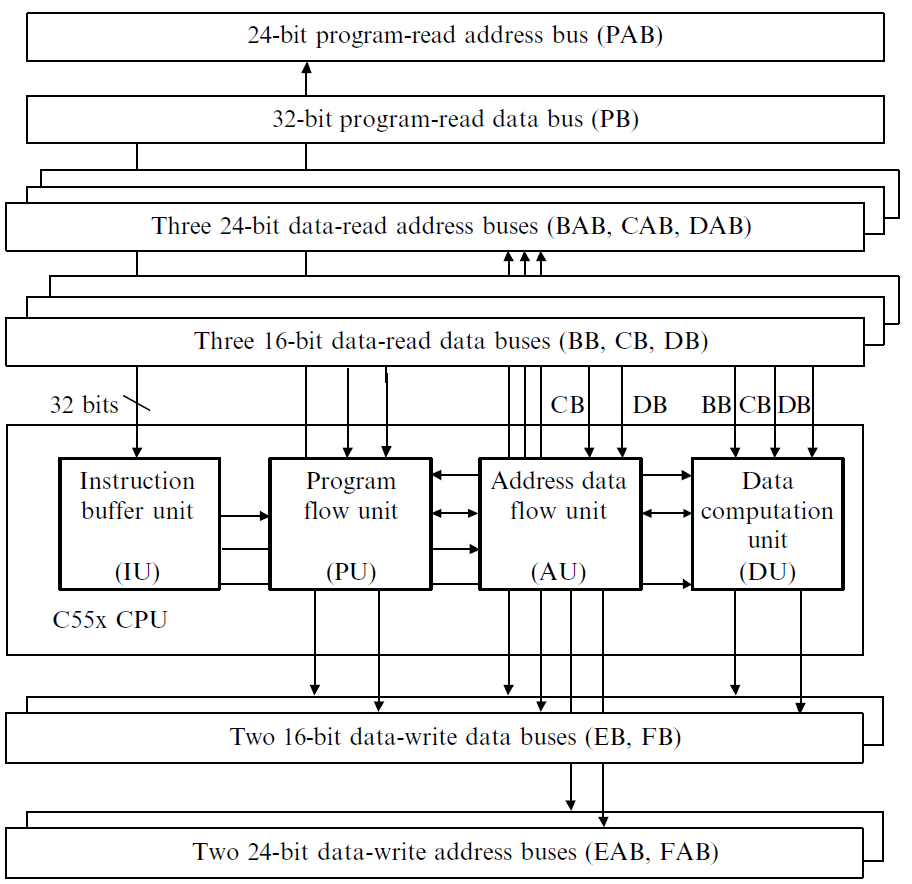
\includegraphics[width=0.7\textwidth]{C2.png}
\caption{Block diagram of the TMS320C55xx CPU.}
\label{fig:DSP}
\end{figure}
The CPU has a harvard strucure which means that data and program memory is seperate. This has the advantage that program and data can fetched and decoded in parallel. The first unit namely the IU, see \autoref{fig:IU}, fecthes instructions from program memory, queues the instructions in an instruction buffer queue and at the same time the instruction decoder decodes an instruction and sends it to the other units.
\begin{figure}[H]
\centering
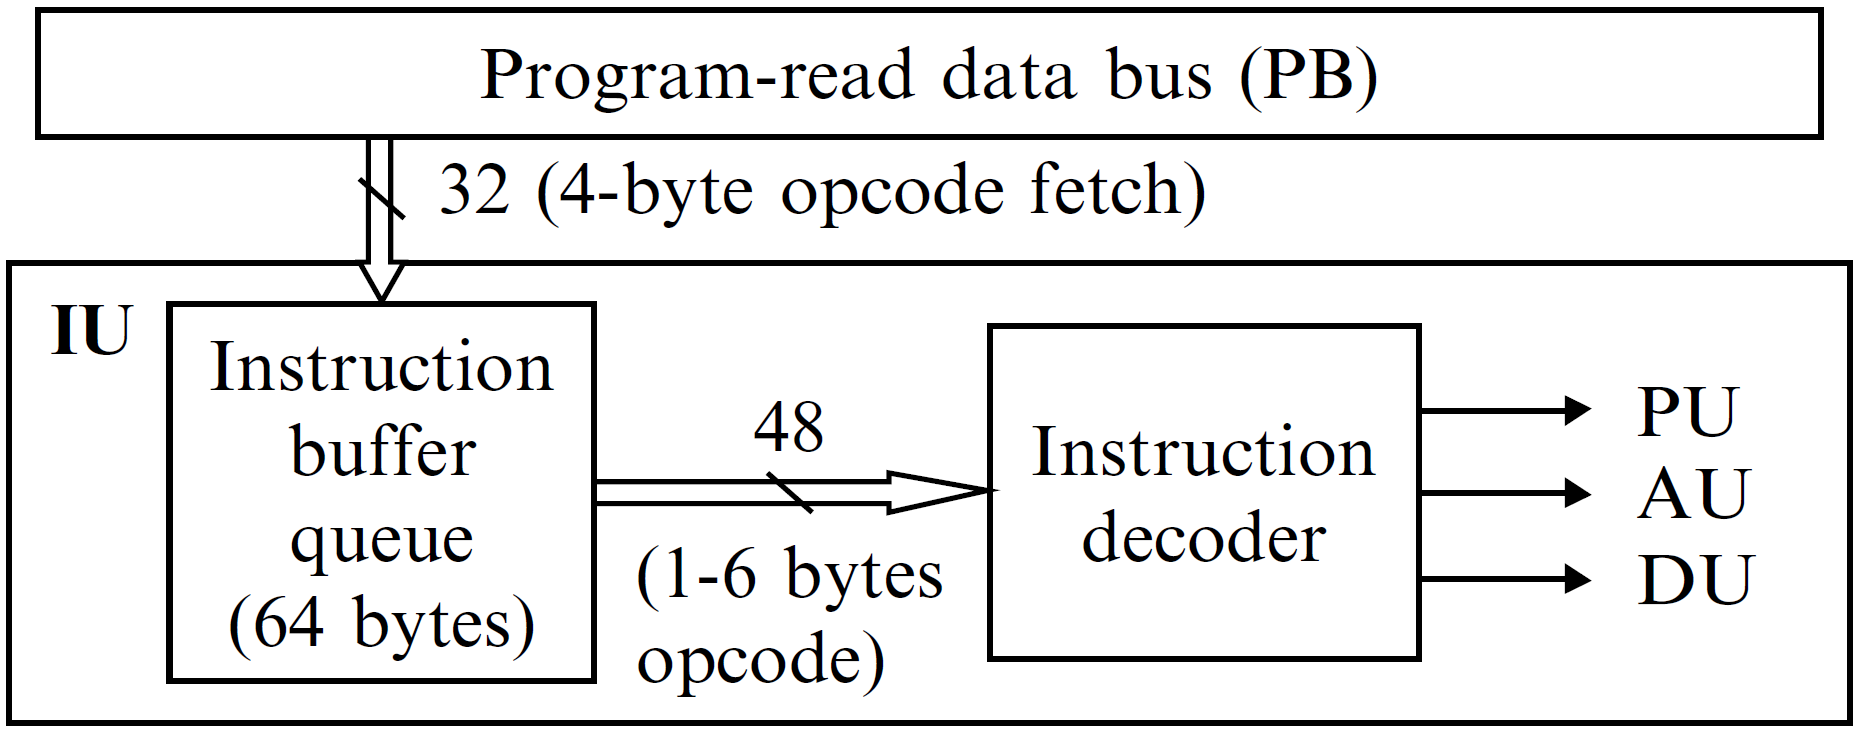
\includegraphics[width=0.5\textwidth]{C1.png}
\caption{Simplified block diagram of the C55xx IU.}
\label{fig:IU}
\end{figure}
The PU, see \autoref{fig:PU}, manages program execution using pipelining for execution efficiency. The program counter (PC) tracks program execution every clock cycle while the adress generator generates a 24 bit adress which 16 Mbytes of memory space. The last component of the PC is the pipeline protection unit which protects the pipeline from non sequential execution such as call, branch or return.
\begin{figure}[H]
\centering
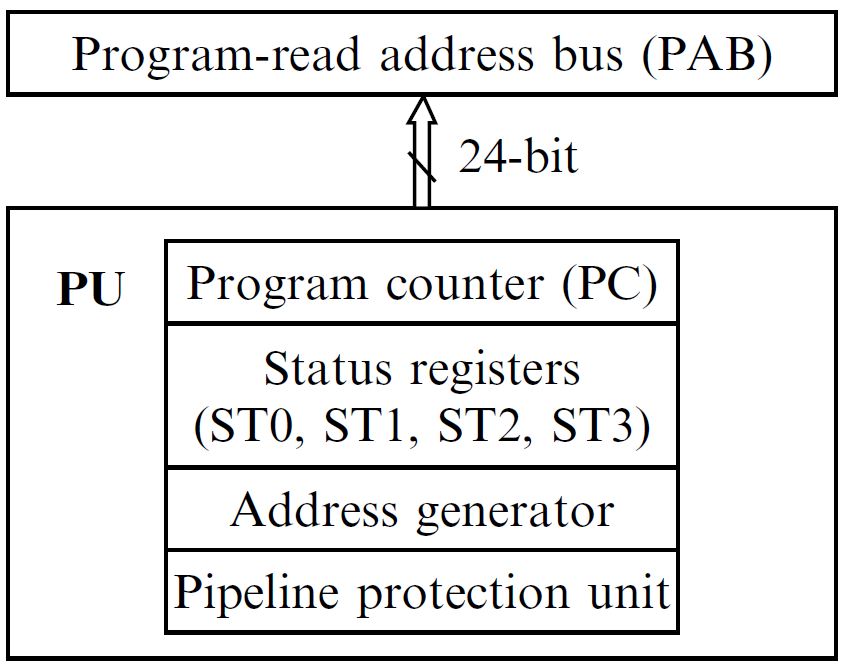
\includegraphics[width=0.4\textwidth]{C0.png}
\caption{Simplified block diagram of the C55xx PU.}
\label{fig:PU}
\end{figure}
The AU, see \autoref{fig:AU}, functions as the data acces manager. The AU consists of eight 23-bit extended auxiliary registers (XAR0-XAR7), four 16-bit temporary registers (T0-T3), a 23-bit coefficient pointer (XCDP), a 23-bit stack pointer (XSP), a 16-bit ALU and can support up to five circular buffers. The AU allows up to two address registers and coefficient pointers working togehter to access two data samples and one coefficient simultaneously in on clock cycle, so parallelity can be used to reduce computation time. 
\begin{figure}[H]
\centering
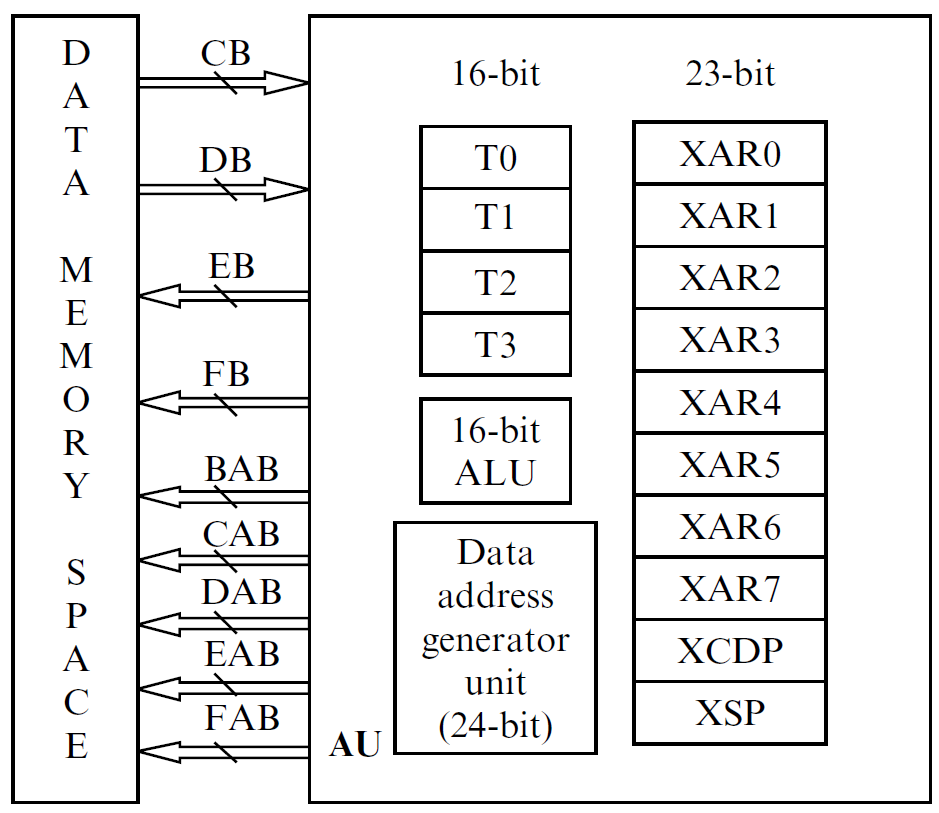
\includegraphics[width=0.5\textwidth]{C4.png}
\caption{Simplified block diagram of the C55xx AU.}
\label{fig:AU}
\end{figure}
The last unit in the CPU is the DU, see \autoref{fig:DU}, which computes data. The DU consists of four accumulators (AC0,AC1,AC2 and AC3), a pair of MAC units, a barrel shifter and rounding and saturation control. There are three data read busses available which allows dual MAC´s access to up to two data paths and a coefficient simultaneously. In one clock cycle each MAC can perform a 17-bit by 17-bit multiplication plus a 40-bit addition/subtraction while the barrel shifter can perform data shifts in the range of $2^{-32}$ to $2^{31}$. 
\begin{figure}[H]
\centering
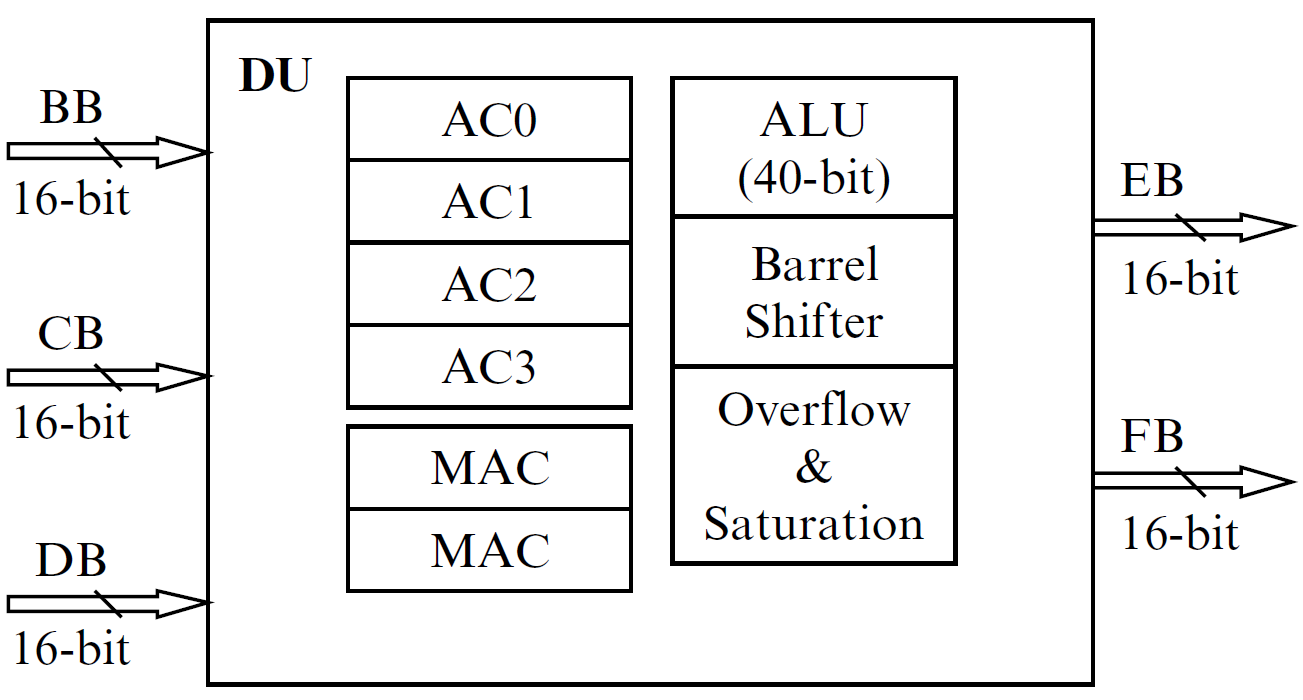
\includegraphics[width=0.5\textwidth]{C5.png}
\caption{Simplified block diagram of the C55xx DU.}
\label{fig:DU}
\end{figure}
This concludes a quick general description of the architecture of the TMS320C55xx which leads to the memory of the CPU. The C55xx on-chip memory has 16Mbytes of memory space which can be used as program or data memory. The on-chip memory consist of of 64Kbyte dual acces ram (DARAM) which is divided into 8Kbyte blocks. DARAM allows C55xx to perform two reads, two writes or one read and one write per clock cycle. The on-chip memory also incudes 256Kbyte single-access RAM (SARAM) divided into 32 blocks of 8Kbyte each, but SARAM only allow for one read or one write per clock cycle.

The two languages used is C and Assembler. They can be used individually or interchangeable. Assembler from a computational view is far superior to C so for computation critical algorithms Assembler should be favored, while C should be favored for overview. This means that C should run the main program and call Assembler functions for computation critical algorithms. 

The reason why C is bad at computational critical algorithms are because the C compiler is a dynamic compiler which does not use the full potential of the instruction set, instead it uses a few defined registers such as SP for example. If an Assembler function is called from C, some specific register are used by the C compiler as input and output data which can be seen on \autoref{fig:CAsm}.
\begin{figure}[H]
\centering
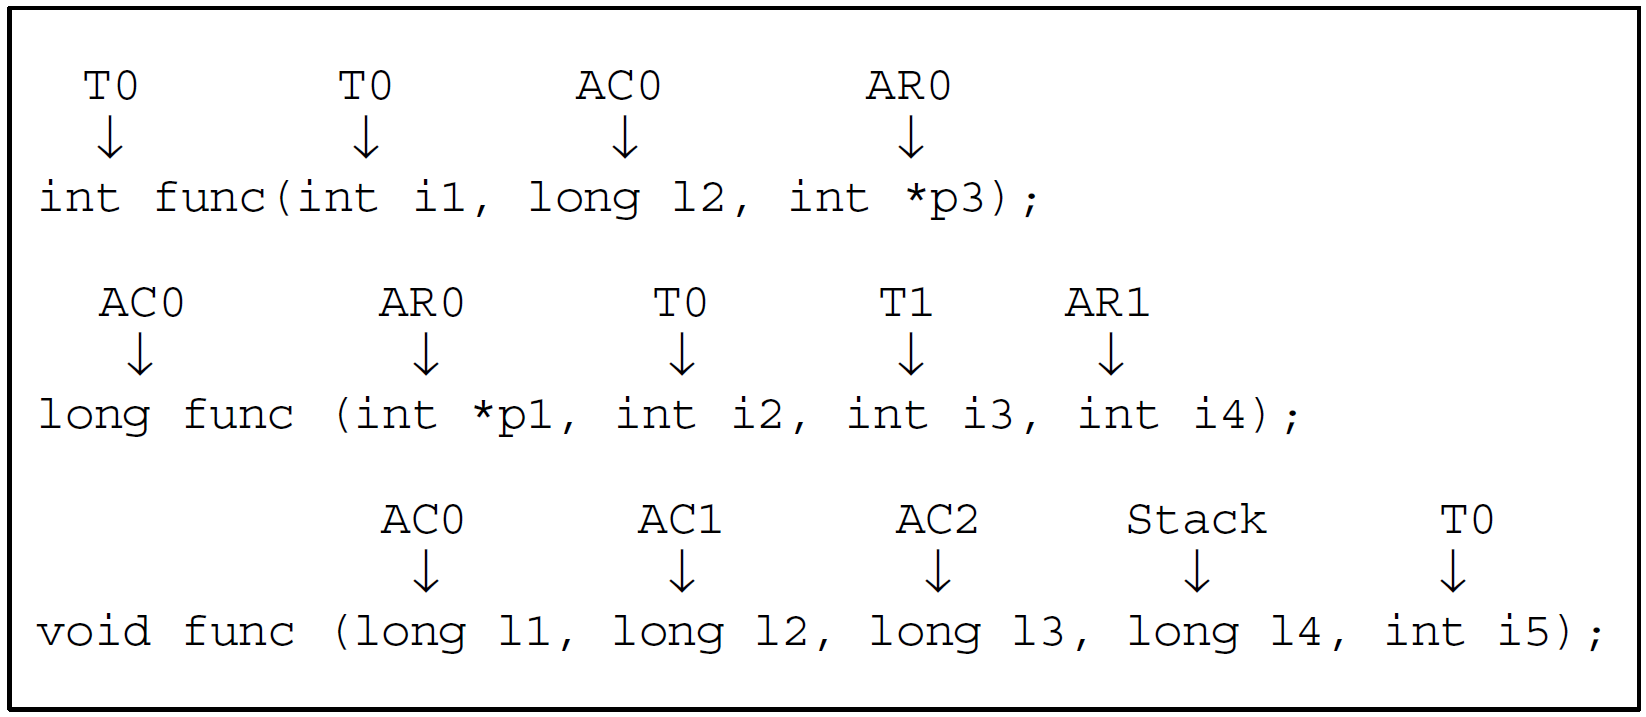
\includegraphics[width=0.8\textwidth]{C6.png}
\caption{Examples of argument-passing conventions.}
\label{fig:CAsm}
\end{figure}
This concludes a quick general description of the CPU which leads to main program.
